\section{Results and Discussion}\label{s:evaluation}
This section reports the interpretation of the experimental results addressing RQ2 and RQ3, evaluated against the hypotheses $H_1$-- $H_3$ defined in Section~\ref{hypotheses}. Standard deviations are reported throughout to characterise the run variability introduced by each coupling strategy. Statistical significance is assessed using a two-sample Welch t-test at $\alpha$ = 0.05. Given the low variance observed in most conditions, the 12\,m acceptance threshold defined in Section~\ref{ss:rqs} is used as the primary basis for interpreting accuracy, with significance testing confirming that observed differences are not attributable to sampling noise.
 

\subsection{Coupling Strategy Comparison and One-Tick Delay Analysis}\label{coupling-results}


Table~\ref{tab:summary} reports the mean apogee height and time as well as wall-clock time over 10 runs per strategy, relative to the RocketPy standalone baseline. 


\begin{table}[h]
\centering
\small
\begin{tabular}{lrrr}
\toprule
\textbf{Mode} & \textbf{Apogee (m)} & \textbf{Apogee Time (s)} & \textbf{Wall Time (s)} \\
\midrule
Non-SIL (baseline)    & 3061.94 $\pm$ 0.00 & 23.49 & 27.0 $\pm$ 1.4 \\
\midrule
SIL Lockstep          & 3061.86 $\pm$ 0.04 & 23.45 & 44.9 $\pm$ 3.8 \\
SIL Snapshot          & 3065.98 $\pm$ 0.03 & 23.46 & 36.4 $\pm$ 2.0 \\
SIL Rate Group 25\,Hz & 3065.78 $\pm$ 0.19 & 23.46 & 36.0 $\pm$ 4.5 \\
\midrule
HIL Lockstep          & 3061.87 $\pm$ 0.03 & 23.45 & 48.8 $\pm$ 3.7 \\
HIL Snapshot          & 3066.00 $\pm$ 0.06 & 23.46 & 41.8 $\pm$ 1.3 \\
HIL Rate Group 25\,Hz & 3069.33 $\pm$ 7.46 & 23.48 & 38.2 $\pm$ 1.7 \\
\bottomrule
\end{tabular}
\caption{Mean apogee ($\pm$ 1 std dev), apogee time, and wall-clock time per coupling strategy, relative to the standalone RocketPy baseline of 3061.94\,m.}
\label{tab:summary}
\end{table}




% \begin{figure}[h]
%     \centering
%     \includegraphics[width=\columnwidth]{figures/results/apogee_bars.png}
%     \caption{Mean apogee per coupling strategy ($\pm$ 1 std dev) across ten runs, with the standalone RocketPy baseline shown as a dashed reference line.}
%     \label{fig:apogee_bars}
% \end{figure}

\subsubsection{Accuracy}
The Lockstep strategy produces the closest apogee to the baseline in both SIL and HIL contexts, with a mean of 3061.86\,m in SIL (-$0.08\,m, $p=0.0001) and 3061.87\,m in HIL (-$0.07\,m, $p=0.0001). Although both are statistically significant, the errors are practically negligible against the acceptance threshold of 12\,m. This is because Lockstep blocks the simulation at every callback until the FSW responds, ensuring that each simulation step uses the actuation output corresponding to the exact sensor reading. It represents an idealised synchronised model that does not exist in real hardware interacting with its environment, but it validates the correctness of flight logic under ideal conditions.

Snapshot produces a consistent overshoot at apogee with a mean of 3065.98\,m in SIL (+$4.04\,m, $p<0.001) and 3066.00\,m in HIL (+$4.06\,m, $p<0.001). The consistency of this overshoot is a structural property of the non-blocking orchestrator design. At callback $n$, the Orchestrator sends the current sensor packet to the FSW and immediately returns the actuation value computed at callback $n-1$ from the actuation buffer, without waiting for the FSW to process the packet from callback $n$. The actuation response corresponding to the callback $n$ is therefore not applied until the callback $n+1$, producing a one-tick delay, where the actuation applied at any callback is always one step behind the sensor reading that triggered it. This delay directly affects the \texttt{AirbrakeController}, as the predicted apogee estimate and the air brake deployment level are always one step behind the true simulation state, causing the PI controller to under-correct during the coasting phase and leading to a systematic overshoot.


The Rate Group strategy at 25Hz produces mean apogee of 3065.78\,m in SIL (+$3.84\,m, $p<0.001) and 3069.33\,m in HIL (+$7.39\,m, $p<0.001). The SIL result exhibits a similar baseline overshoot to Snapshot, consistent with both strategies sharing the same non-blocking simulation behaviour. Both Rate Group SIL and HIL apogee accuracy show higher variance than Snapshot, since \texttt{FlightMain} runs on its own independent clock, decoupled from RocketPy's callback function, meaning that the actuation buffer at any given callback may represent a value computed on a different tick. In HIL, this variance increases further, reaching 7.46\,m compared to 0.19\,m in SIL, as the difference between the two independent clocks compounds with the reduced CPU performance of the target hardware and added Ethernet latency. Together with the Lockstep and Snapshot results above, these findings confirm $H_1$, as Lockstep, which enforces synchronisation, produces negligible overshoot, while both non-blocking strategies, Snapshot and Rate Group, introduce a one-tick delay that causes a consistent apogee overshoot in both SIL and HIL.

All three strategies, however, remain within the 12 m acceptance threshold in both SIL and HIL, confirming that each is suitable for pre-flight validation despite their architectural differences.

The nature of this one-tick delay was further confirmed by running an informal check against a second rocket configuration (not part of the controlled experiments), in which the overshoot magnitude differed, but the delay persisted across both non-blocking strategies, confirming that it is a property of the Orchestrator design rather than the rocket configuration. The timing behaviour produced by this delay is representative of real embedded flight software execution. On real hardware, sensor readings will always be slightly stale by the time they are processed on a fixed hardware clock. 

Table~\ref{tab:deployment_timings} reports the parachute deployment times according to each strategy. Lockstep and Snapshot deploy the drogue at $t \approx 25.00$\,s across both SIL and HIL execution contexts, and the main parachute at $t \approx 44.60$\,s. The Rate Group strategy shows earlier drogue deployment at $24.84$\,s (SIL) and $24.91$\,s (HIL), but with higher variance in both drogue and main times consistent with its timing non-determinism.

\begin{table}[htbp]
\centering
\small
\begin{tabular}{lrrr}
\toprule
\textbf{Deployment} & \textbf{Drogue Parachute (s)} & \textbf{Main Parachute (s)} \\
\midrule
Non-SIL (baseline)   & $25.00 \pm 0.00$ & $44.60 \pm 0.00$ \\
\midrule
SIL Lockstep         & $25.00 \pm 0.00$ & $44.60 \pm 0.00$ \\
SIL Snapshot         & $25.00 \pm 0.01$ & $44.60 \pm 0.00$ \\
SIL Rate Group 25 Hz & $24.84 \pm 0.04$ & $45.18 \pm 0.25$ \\
\midrule
HIL Lockstep         & $25.01 \pm 0.00$ & $44.64 \pm 0.01$ \\
HIL Snapshot         & $25.01 \pm 0.00$ & $44.64 \pm 0.01$ \\
HIL Rate Group 25 Hz & $24.91 \pm 0.07$ & $45.09 \pm 0.28$ \\
\bottomrule
\end{tabular}
\caption{Mean parachute deployment timings and standard deviations per coupling strategy. Measured in simulation time $t$.}
\label{tab:deployment_timings}

\end{table}


\subsubsection{Wall-Clock Time}
Wall-clock time distributions are shown in Table \ref{tab:summary} and illustrated in Figure \ref{fig:wall_time_violin}. The stand-alone baseline completes in 27.0\,$\pm$\,1.4\,s, and all coupling strategies introduce overhead relative to it. Among SIL configurations, Lockstep is the slowest at 44.9\,$\pm$\,3.8\,s, while Snapshot and Rate Group are comparable at 36.4\,$\pm$\,2.0\,s and 36.0\,$\pm$\,4.5\,s, respectively. HIL configurations are slower than their SIL  counterparts across all strategies, with HIL Lockstep the slowest overall at 48.8\,$\pm$\,3.7\,s, followed by HIL Snapshot at 41.8\,$\pm$\,1.3\,s and HIL Rate Group at  38.2\,$\pm$\,1.7\,s.

\begin{figure}[h]
    \centering
    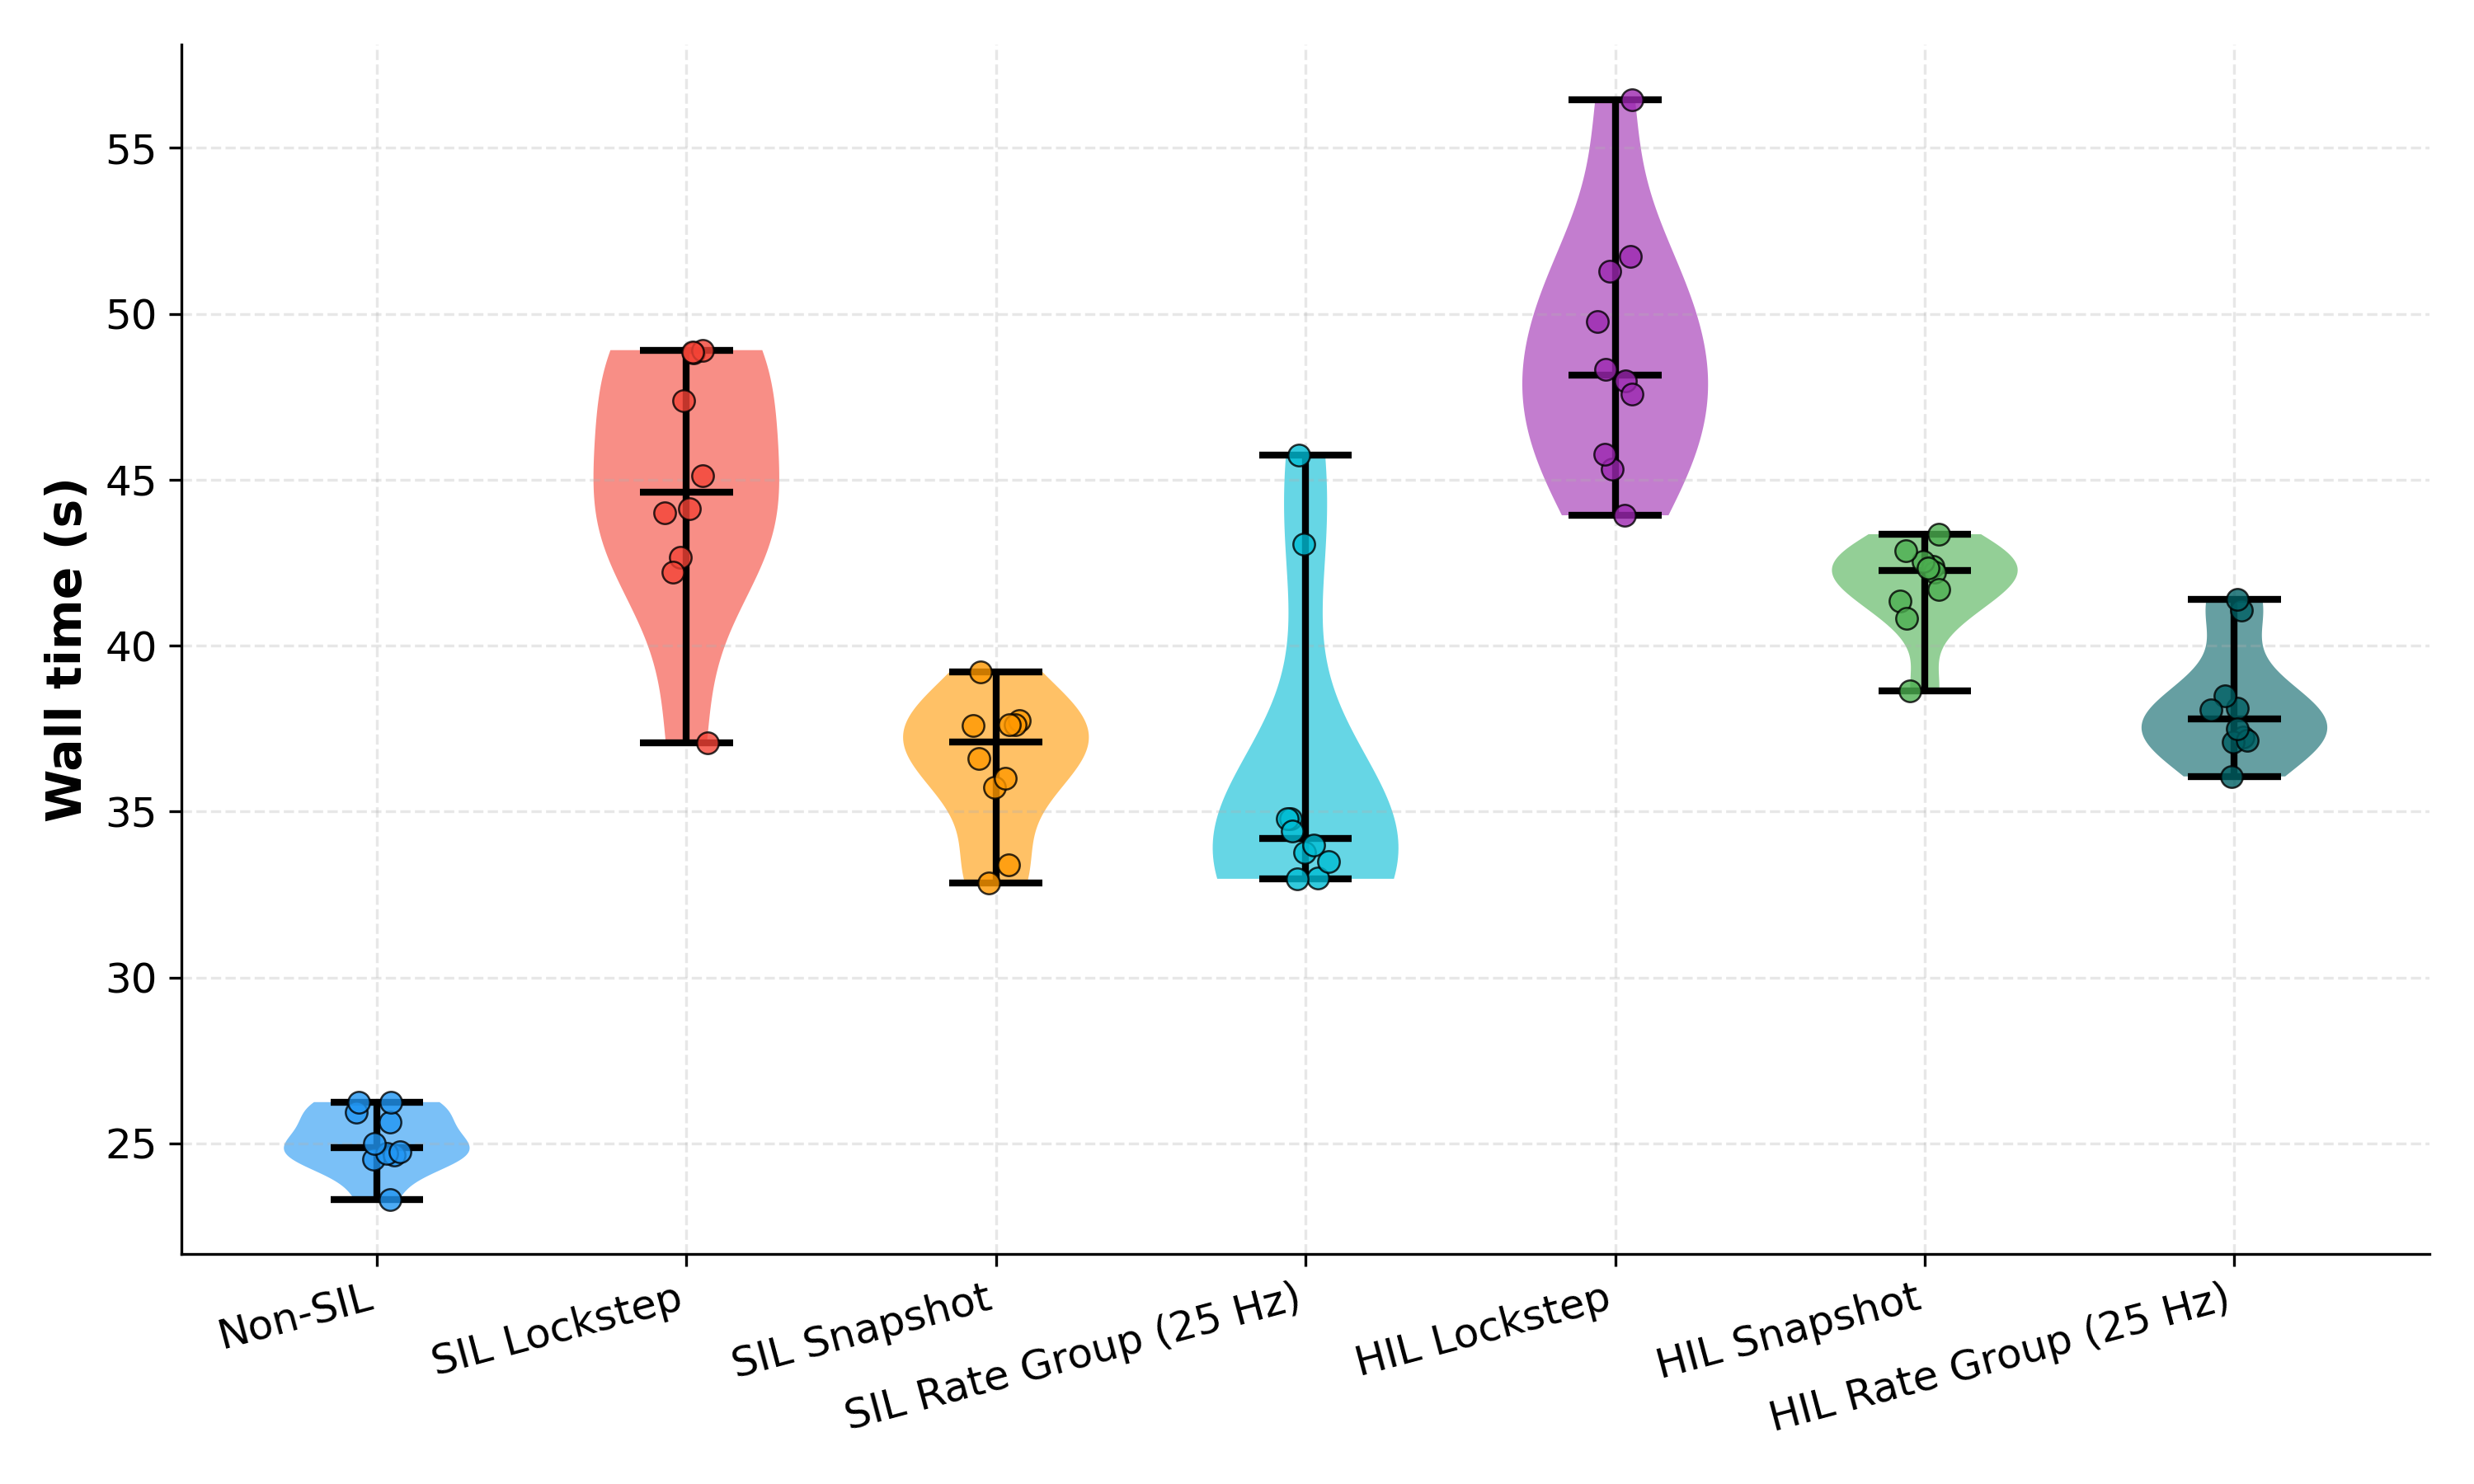
\includegraphics[width=\columnwidth]{figures/results/wall_time_violin.png}
    \caption{Wall-clock time distribution per coupling strategy.}
    \label{fig:wall_time_violin}
\end{figure}
For Lockstep, the overhead is most notable in both contexts due to its blocking nature. The additional cost in HIL relative to SIL (48.8\,s versus 44.9\,s) is attributed to the Ethernet round-trip between the host and the Raspberry Pi 4, as well as the reduced CPU performance of the target hardware, which extends the processing time of the FSW. For the Snapshot and Rate Group strategies, neither block the simulation, so the additional overhead is attributed to just the Ethernet transmission latency, as reflected in the smaller but consistent gap in wall-clock times. These results confirm $H_2$: HIL configurations produce longer wall-clock times than their SIL counterparts, attributable to Ethernet latency and reduced CPU performance on the target hardware.






% \subsection{SIL vs HIL Agreement}\label{sil-hil-results}

\subsection{Rate Group Frequency Sweep}\label{freq-sweep}
Figure~\ref{fig:rate-apogee-freq} shows the mean apogee as a function of \texttt{RateGroupDriver} tick frequency with SIL and HIL combined. At 1Hz, the mean apogee reaches 3271.5\,$\pm$\,59.0\,m; this is an overshoot of 209.56\,m, as the FSW uses stale data and transmits air brake actuations only once per second, too infrequently to efficiently track the coasting dynamics. A clear trend is evident: the error decreases monotonically with frequency, from 101.19\,m at 5\,Hz, to 27.69\,m at 10\,Hz, to 5.61\,m at 25\,Hz, to 4.0\,m at 50\,Hz. This is because at higher tick frequencies, the FSW reads more recent sensor data and actuates more frequently, reducing the window of stale data between ticks and allowing the \texttt{AirbrakeController} to track the trajectory with higher accuracy. The diminishing accuracy gains beyond 25\,Hz informed the selection of this frequency for the comparison of coupling strategies in Section~\ref{coupling-results}.

\begin{figure}[h]
    \centering
    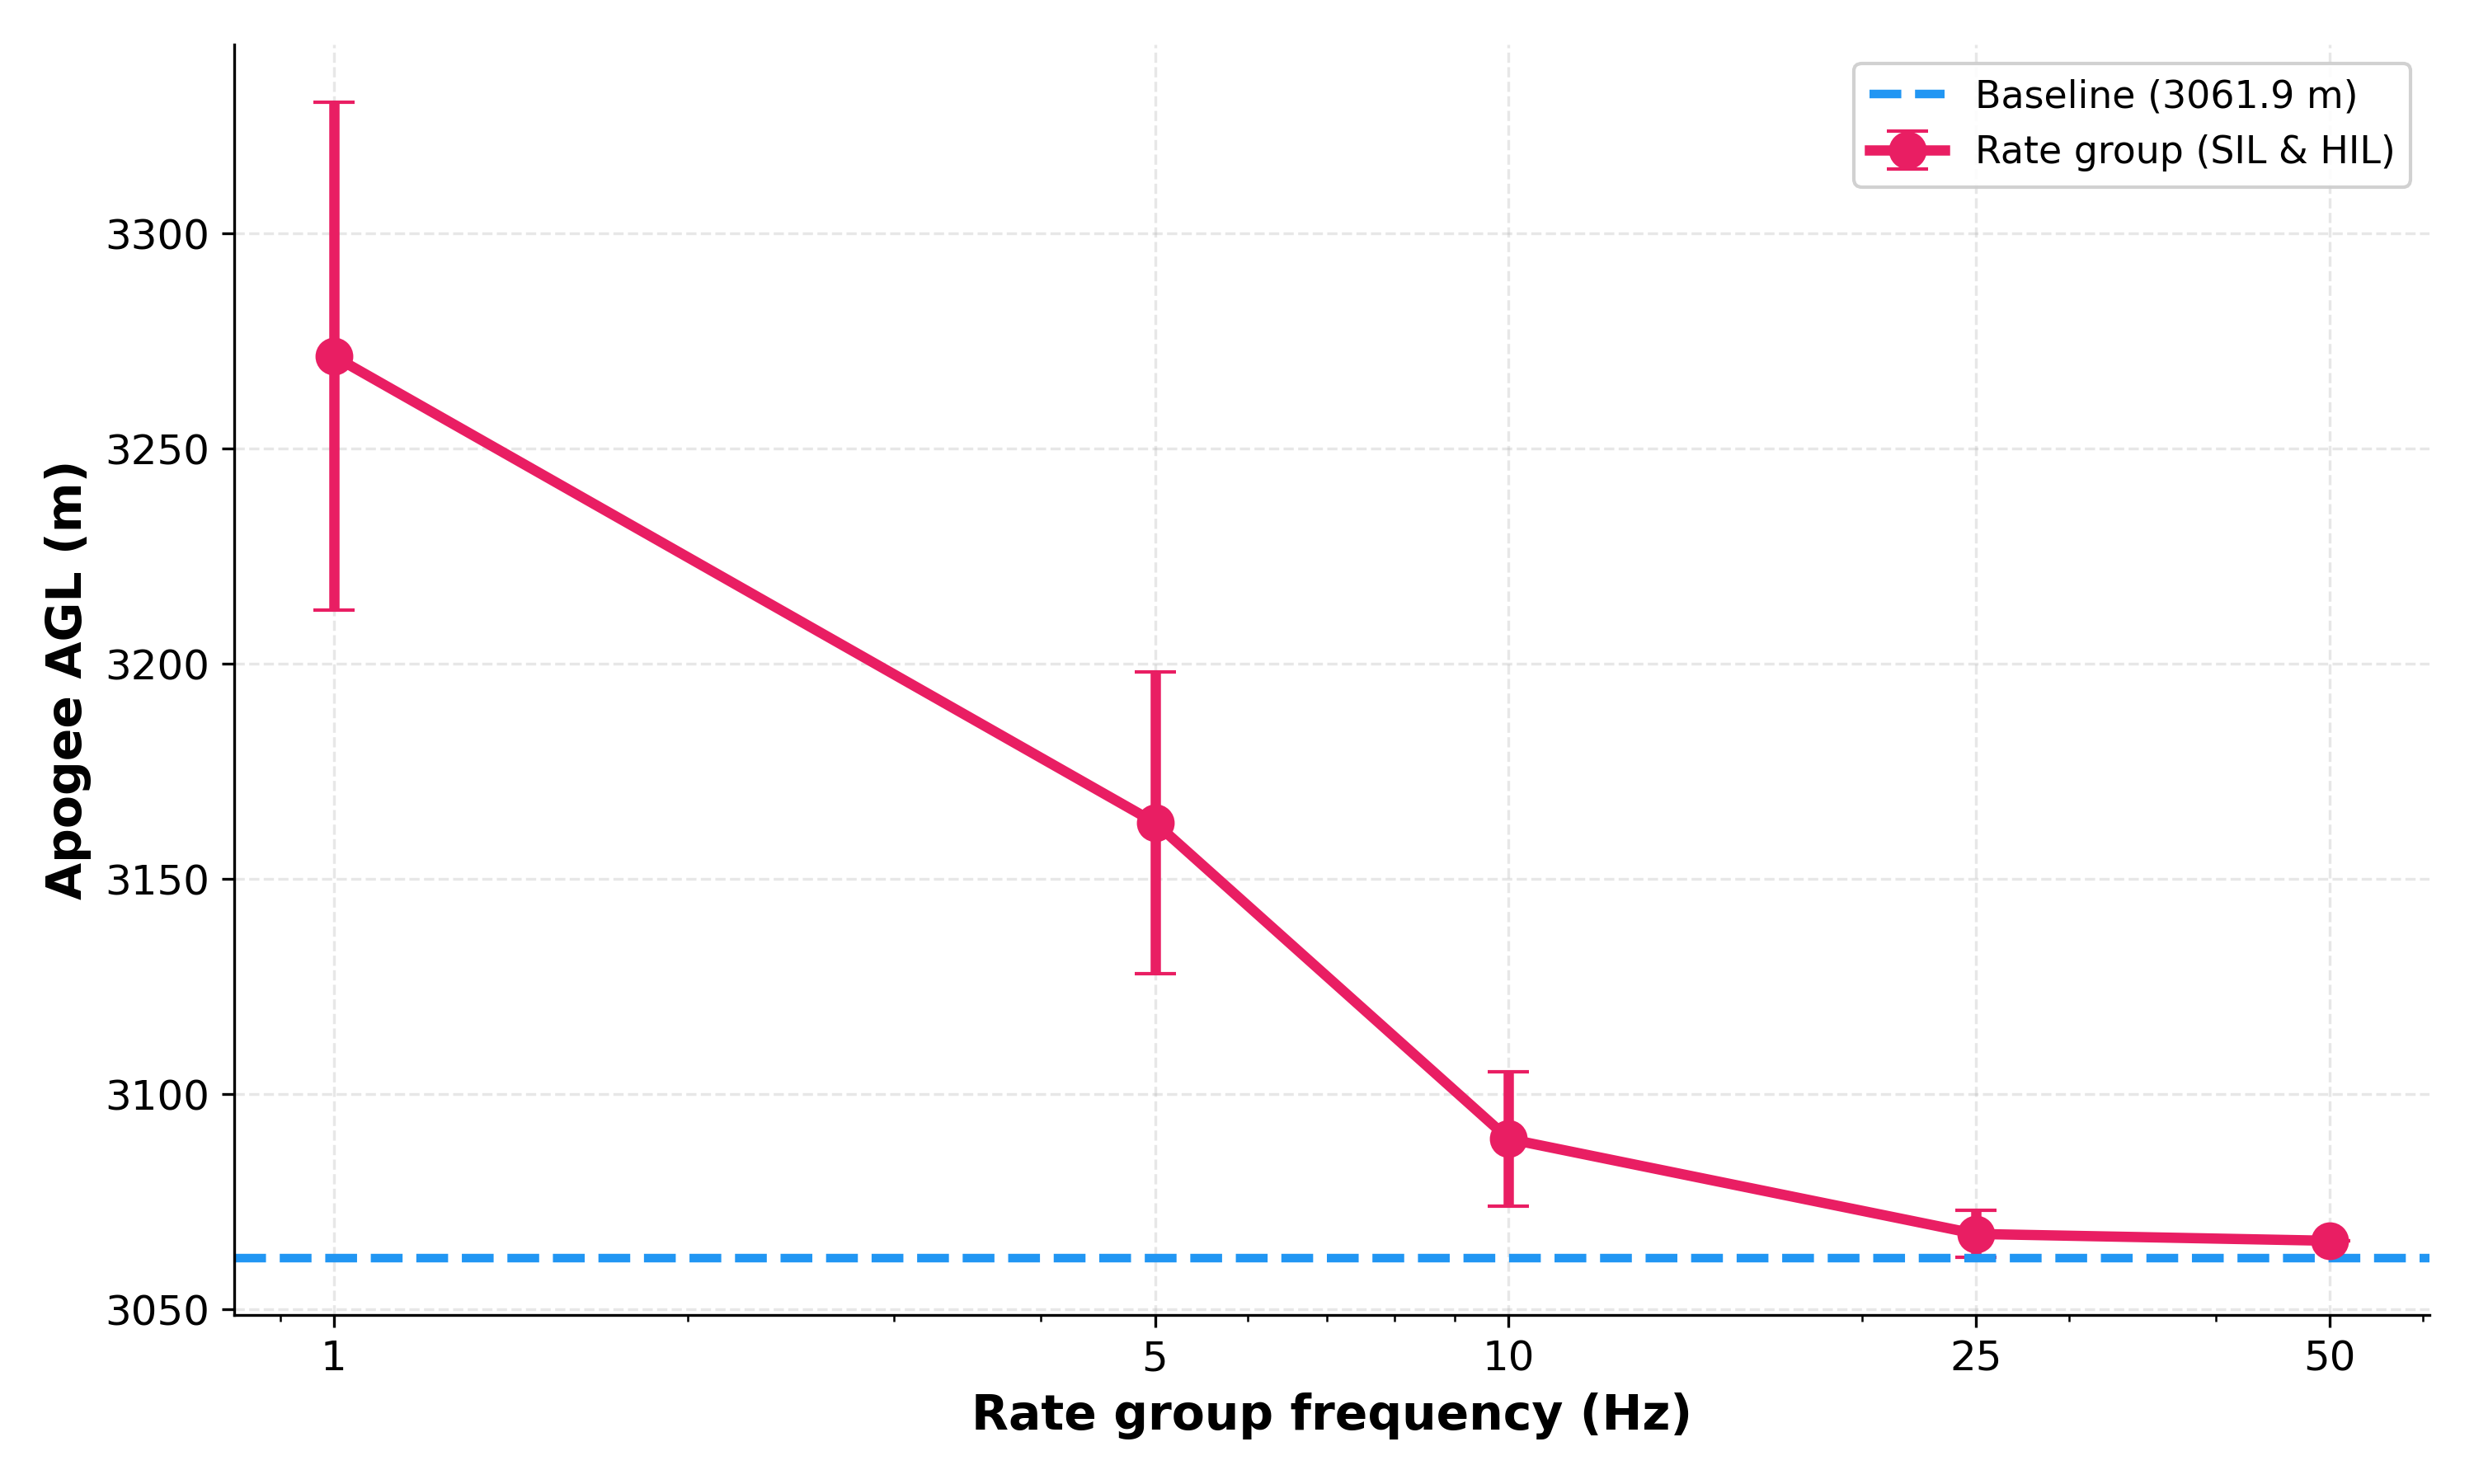
\includegraphics[width=\columnwidth]{figures/results/rategroup_apogee_vs_freq.png}
    \caption{Mean apogee as a function of Rate Group tick frequency, SIL and HIL combined.}
    \label{fig:rate-apogee-freq}
\end{figure}



\subsection{Fault Injection}\label{fault-results}
Figure \ref{fig:fault_injection} illustrates the trajectory and FSW events during the fault injection scenario across all 20 runs (SIL and HIL). At $t = 10$\,s, a barometric freeze is injected during the coasting phase, causing the perceived altitude of the FSW to be held at approximately 1995\,m. The fault-recovery logic explained in Section~\ref{flight-logic} detects this freeze at $t$=11.5\,s and switches to IMU-based apogee detection. The rocket reaches a true apogee of 3069\,m at $t$=23.5\,s. The drogue parachute is deployed at $t$=23.6\,s (SIL) and $t$=23.61\,s (HIL), placing deployment 0.1\,s after true apogee, compared to a 1.54\,s delay under nominal barometric detection at the same Snapshot apogee time reported in Table~\ref{tab:summary} ($t$=23.46\,s, drogue at $t$=25.0\,s). The main parachute deploys at $t$=43.60\,s in both contexts, 20\,s after drogue deployment, via the \texttt{MAIN\_DEPLOY\_TIMEOUT} fallback. These results confirm $H_3$: the FSW successfully detected the sensor fault and deployed the drogue parachute near apogee in both execution contexts.

\begin{figure}[h]
    \centering
    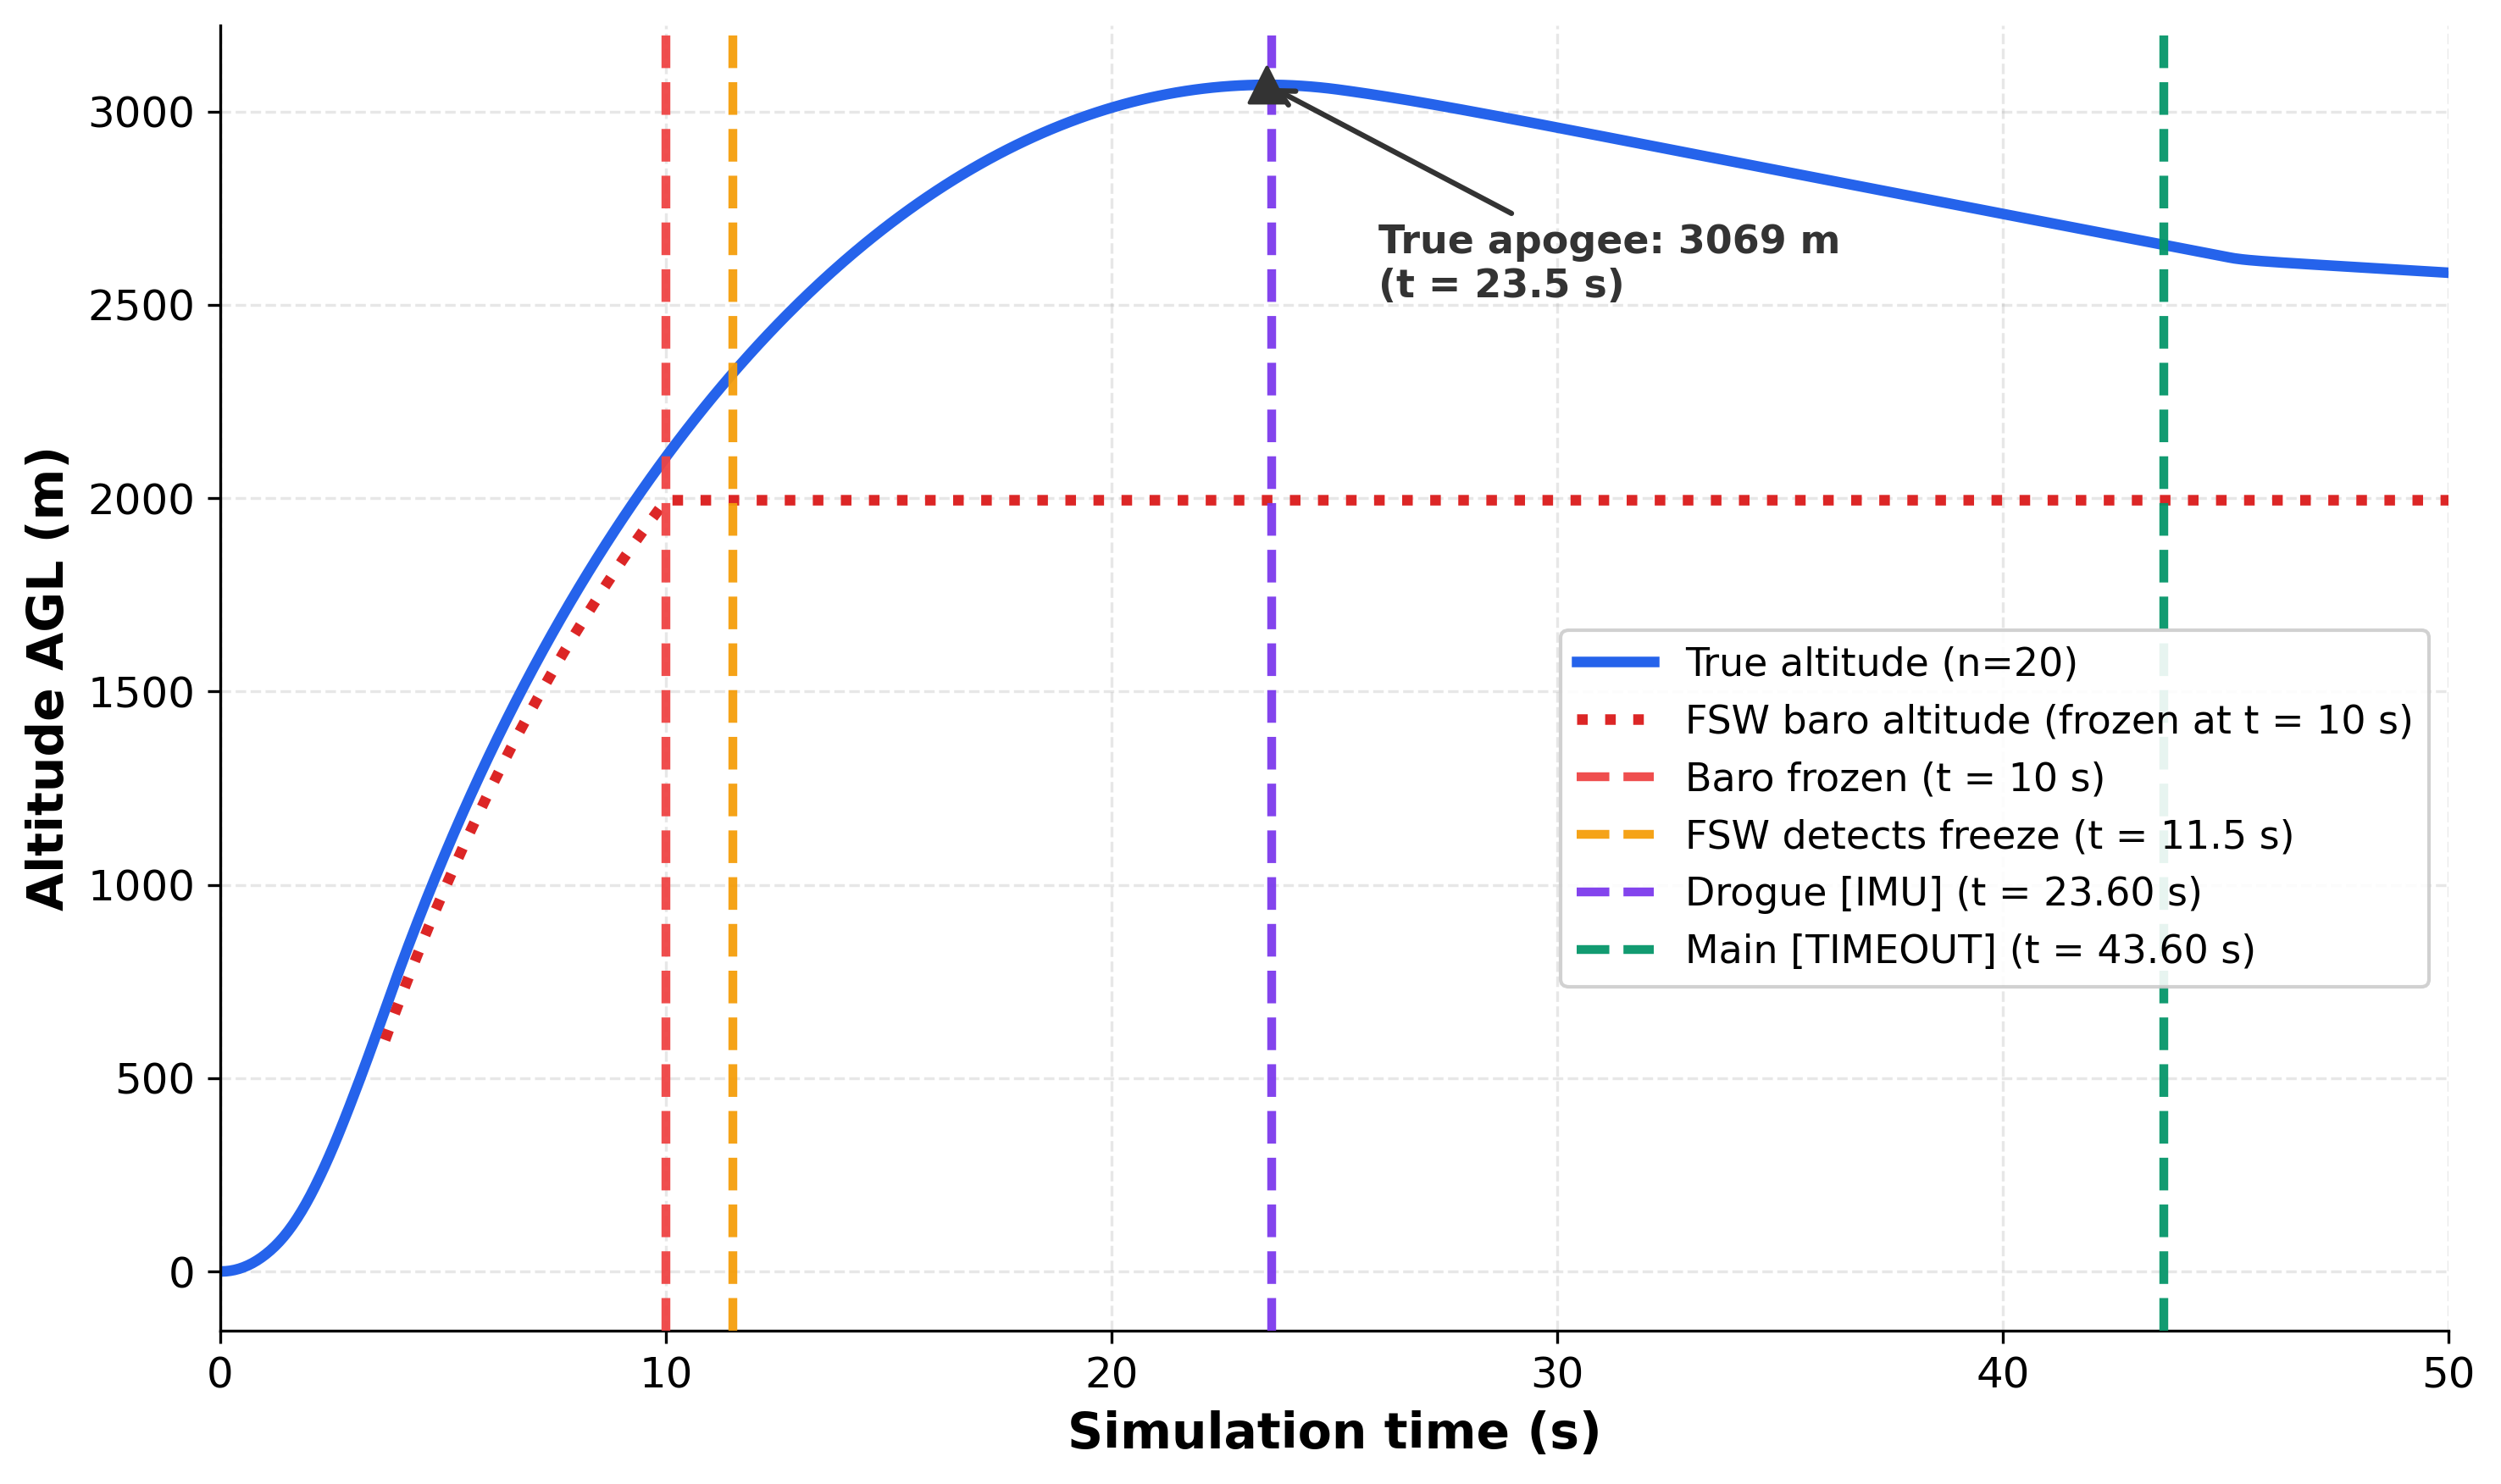
\includegraphics[width=\columnwidth]{figures/results/fault_injection.png}
    \caption{Fault injection experiment, showing the trajectory and FSW events across all 20 runs. The barometric freeze at $t$ = 10\,s triggers IMU-based fallback detection and drogue deployment 0.1 s after true apogee.}
    \label{fig:fault_injection}
\end{figure}

Notably, the IMU-based fallback logic deployed the drogue significantly closer to apogee than the nominal barometric detection. Under no-fault conditions, drogue deployment occurred 1.54\,s after apogee, while the fallback path reduced this gap by 1.44\,s.

This unintentional finding further demonstrates the value of closed-loop testing in flight software development. This result could not have been observed through open-loop testing, as it depends on the FSW to feed the actuation output back into the simulation state. The slight apogee overshoot of 3069\,m relative to the nominal Snapshot apogee of 3066\,m is a separate consequence of the barometric freeze. With altitude held constant, the \texttt{AirbrakeController} can no longer compute a valid predicted apogee, causing under-deployment of the air brakes during the coasting phase.

The difference in detection performance stems from the 10-consecutive-pressure-reading confirmation window for barometric detection. In contrast, IMU-based detection responds as soon as vertical acceleration drops below \texttt{ACCEL\_FREEFALL\_THRESH}, a condition satisfied within one callback call at apogee. The main parachute was deployed at $t=43.60$\,s in both SIL and HIL, exactly $20$\,s after drogue deployment, through the \texttt{MAIN\_DEPLOY\_TIMEOUT} fallback, confirming that the complete recovery sequence was completed under faulty-sensor conditions.

\subsection{Controller Callback Sample Rate Sweep} \label{callback-sample-rate}
Figure \ref{fig:callback-sweep-by-strategy} shows the mean apogee as a function of the controller callback sampling rate for the Non-SIL baseline, Lockstep and Snapshot strategies, with an average taken for SIL and HIL, as the two execution contexts produced near-identical results at every rate. 

Figure \ref{fig:callback-sweep-by-strategy} demonstrates that Lockstep matches the baseline closely across every tested rate (within $\sim 0.1$\,m), consistent with its zero-tick delay design, confirmed in Section \ref{coupling-results}. As expected, due to the one-tick delay, Snapshot consistently overshoots. This overshoot decreases as the sampling rate increases, from approximately 4.8\,m at 5\,Hz to 1.3\,m at 50\,Hz, with the largest reduction occurring between 10\,Hz and 25\,Hz (4.2\,m to 1.9\,m). This indicates that the one-tick delay's practical impact on apogee accuracy diminishes as the controller is invoked more frequently.

Notably, both the baseline and Lockstep show a small, shared non-monotonicity, rising slightly at 25 Hz relative to 10 Hz before decreasing again at 35 and 50 Hz. Since this appears identically in the Non-SIL baseline, which involves no coupling, Orchestrator, or FSW, it cannot be attributed to the one-tick delay or any other coupling effect. It instead reflects the PI controller's own sensitivity to discretisation at different sampling rates.

A brief check of solver time-step sensitivity found apogee remaining within 0.1\,m of the default across time steps of 0.001, 0.005 and 0.01 s for both the Non-SIL baseline and Snapshot, with wall-clock time decreasing as the step widened. A single run at a much finer step of 0.0001 s increased wall-clock time considerably, rising to 237\,s, but produced only a marginal apogee change (3066.8 m versus 3066.0 m), suggesting the one-tick delay has negligible sensitivity to the solver computational load within the range tested. A fuller repeated sweep was outside the scope of this study.

\begin{figure}[h]
    \centering
    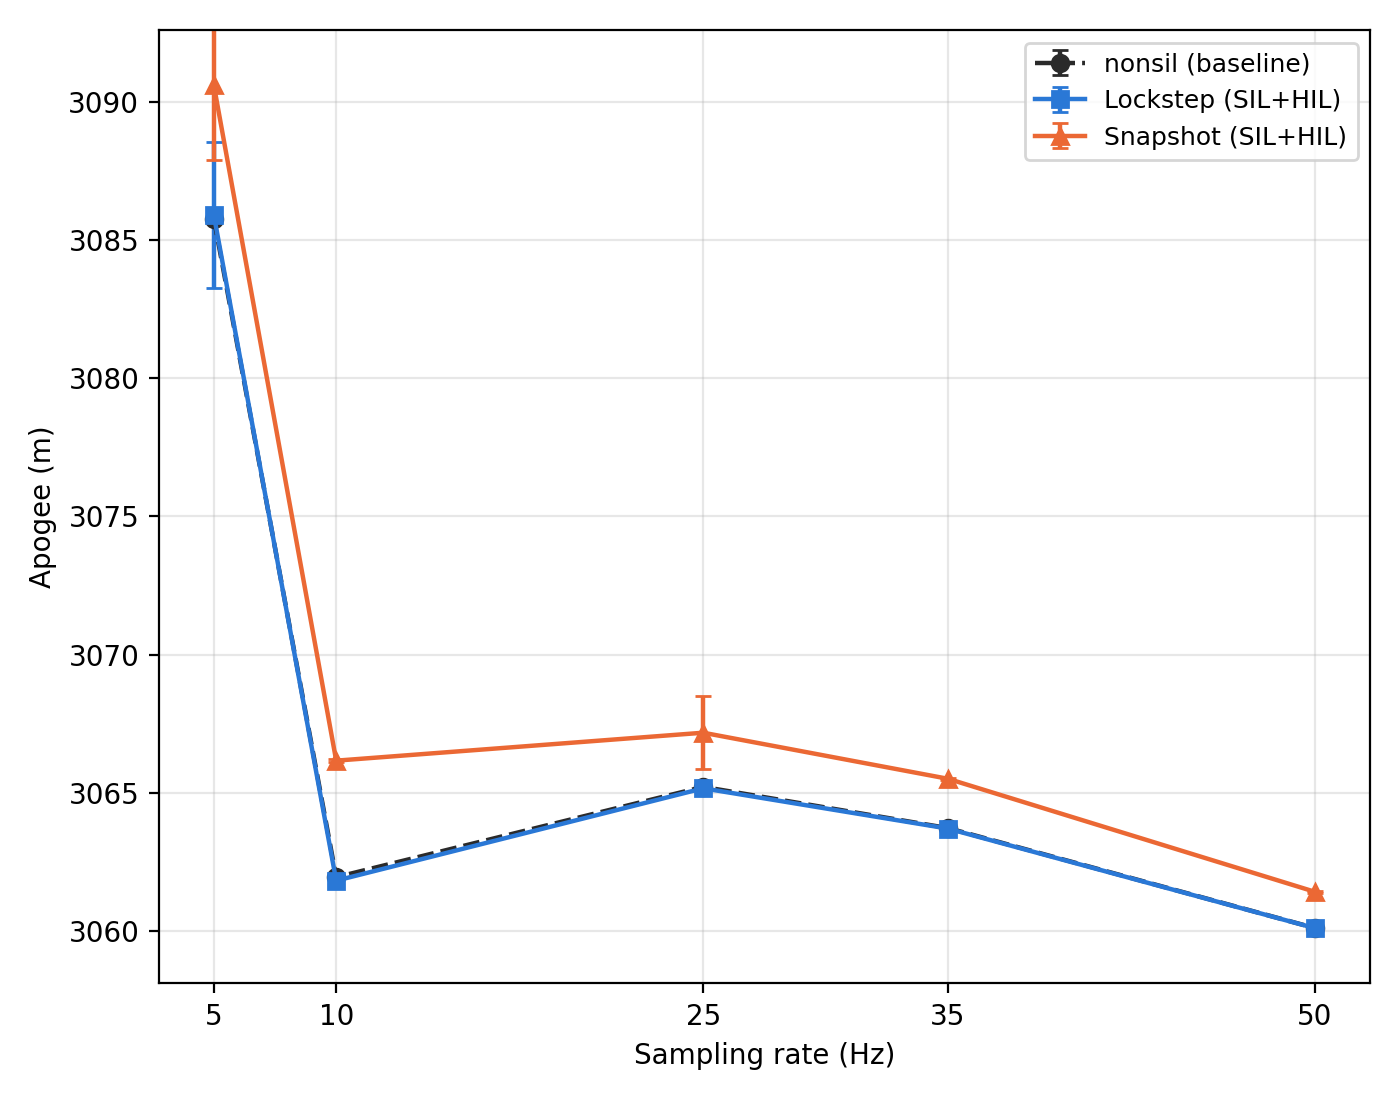
\includegraphics[width=\columnwidth]{figures/results/apogee_by_strategy.png}
\caption{Mean apogee as a function of controller callback sampling rate for the Non-SIL baseline, Lockstep and Snapshot strategies (SIL and HIL combined).}    \label{fig:callback-sweep-by-strategy}
\end{figure}



These results answer RQ2 and RQ3. Coupling strategy and execution context measurably affect apogee accuracy, deployment timing and wall-clock overhead ($H_1$, $H_2$), yet all three strategies remain within the pre-flight acceptance threshold of 12\,m in both SIL and HIL. The fault injection results confirm $H_3$: the framework successfully injects a representative sensor fault, and the FSW recovers in both execution contexts.

% \begin{table}[h]
% \centering

% \label{tab:ttest}
% \small
% \begin{tabular}{lrrr}
% \toprule
% \textbf{Comparison} & \textbf{$t$} & \textbf{$p$} & \textbf{Significant} \\
% \midrule
% Baseline vs SIL Lockstep       &   6.311  & 0.0001   & Yes \\
% Baseline vs HIL Lockstep       &   7.139  & 0.0001   & No  \\
% Baseline vs SIL Snapshot       & $-$393.6 & $<$0.001 & Yes \\
% Baseline vs HIL Snapshot       & $-$218.1 & $<$0.001 & Yes \\
% Baseline vs SIL Rate Group 25\,Hz & $-$63.8 & $<$0.001 & Yes \\
% Baseline vs HIL Rate Group 25\,Hz & $-$3.132 & 0.012  & Yes \\
% \bottomrule
% \end{tabular}
% \caption{Welch $t$-test results comparing each coupling strategy against 
% the standalone baseline. Significance assessed at $\alpha = 0.05$.}
% \end{table}






% \begin{figure}[h]
%     \centering
%     \includegraphics[width=\columnwidth]{figures/results/parachute_timing.png}
%     \caption{Drogue and Main trigger time per coupling strategy.}
%     \label{fig:drogue-timing}
% \end{figure}



% \subsection{Architecture Comparison (RQ1 \& RQ2)}

% Table~\ref{tab:summary} reports mean apogee and wall-clock time across ten runs per mode, relative to the standalone RocketPy baseline of 3061.89~m. Figure~\ref{fig:apogee_bars} shows apogee per mode and Figure~\ref{fig:wall_time} shows wall-clock 
% time distributions.

% \subsubsection{RQ 1: Accuracy}
% The lockstep architecture is the closest in similarity to the baseline in both execution contexts. SIL Lockstep produces a mean apogee of 3061.86~m, and HIL Lockstep 3061.87~m, resulting in errors of just $-0.03$ and $0.02$~m respectively. 

% Snapshot architecture produces a consistent overshoot of approximately 4.1~m in both SIL and HIL, with 

% \subsection{SIL Vs HIL (RQ3)}
% \subsection{Rate Group Frequency Sensitivity (RQ4)}
% \subsection{Fault Injection and Recovery (RQ5)}
% \TODO{
% Discuss the design of your experiments, the results you obtained, and how they
% help in evaluating the claims you made in the introduction. You may also use the
% evaluation results in this section to justify your design choices or assess the
% contributions of different aspects  of your design towards the overall goals.
% }



